%
% This work is licensed under a Creative Commons Attribution-ShareAlike 4.0 International License.
% http://creativecommons.org/licenses/by-sa/4.0/
%

% DO NOT COMPILE THIS FILE DIRECTLY!
% This is included by the other .tex files.


\begin{frame}
    \includegraphics[scale=0.3]{images/logo-circl-Forensics.png}
    \begin{itemize}
        \item[]
        \item[]
        \item[] 7. Memory Forensics
    \end{itemize}
\end{frame}


\begin{frame}
  \frametitle{7.1 About Memory Forensics}
    \begin{itemize}
        \item History
            \begin{itemize}
                \item 2005: String search
		\item $\to$ EProcess structures
		\item[]
            \end{itemize}
        \item Finding EProcess structures
            \begin{itemize}
		\item Find the doubly linked list (ntoskrnl.exe)
		\item Brute Force searching
		\item[]
            \end{itemize}
        \item Information expected
            \begin{itemize}
		\item Processes (hidden)
		\item Services (listening)
                \item Malware
                \item Network connections
                \item Registry content
                \item Passwords
                \item Cleartext data
		\item[]
            \end{itemize}
    \end{itemize}
\end{frame}


\begin{frame}
  \frametitle{7.2 Capturing memory}
    \begin{itemize}
        \item Prepare USB device
            \begin{itemize}
                    \item[] File system: ExFAT; NTFS
                    \item[] Executable capturing tool
                    \item[] No installation - Little impact as possible
                    \item[] Write capture on device
                    \item[] Administrator privileges required
                    \item[]
            \end{itemize} 
        \item Capture memory from running system
            \begin{itemize}
                    \item[] DumpIt.exe
                    \item[] \texttt{DumpIt.exe} part of Comae-Toolkit
                    \item[] \url{https://www.comae.com/}
                    \item[] \url{https://github.com/Crypt2Shell/Comae-Toolkit/}
                    \item[] 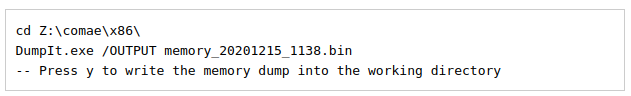
\includegraphics[scale=0.55]{images/dumpCmd.png}
                    \item[]
            \end{itemize} 
    \end{itemize}
    % 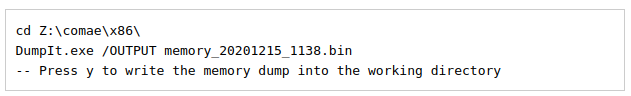
\includegraphics[scale=0.55]{images/dumpCmd.png}
\end{frame}


\begin{frame}
  \frametitle{7.2 Capturing memory}
      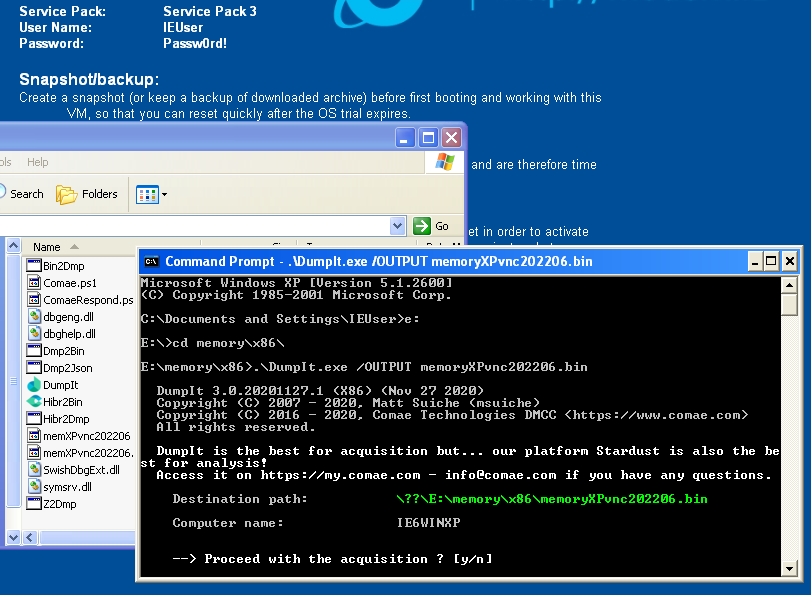
\includegraphics[scale=0.36]{images/dumpIt.png}
\end{frame}


\begin{frame}
  \frametitle{7.2 Capturing memory}
    \begin{itemize}
        \item Hibernation file: \texttt{hiberfil.sys}
            \begin{itemize}
		    \item[] Created when going into hibernation mode
		    \item[] Fully fleded memory content
		    \item[] Compressed and slightly modified
		    \item[] Can be converted into raw memory dump
		    \item[] Force hibernation:
                    \begin{itemize}
		        \item[] \texttt{powercfg /h[ibernate] [on|off]}
		        \item[] \texttt{psshutdown -h}
                    \end{itemize}
            \end{itemize}
        \item[]
        \item Pagefile: \texttt{pagefile.sys}
        \item[]
	\item Swapfile: \texttt{swapfile.sys} (Windows 8)
        \item[]
	\item Crash dump: \texttt{memory.dmp} (Blue Screen)
        \item[]
    \end{itemize}
\end{frame}


\begin{frame}[fragile]
  \frametitle{7.3 BulkExtractor Exercise}
    \begin{lstlisting}[basicstyle=\tiny]
1. Preparation
--------------

    sudo mount -o ro,offset=$((512*2048)) circl-dfir.dd /media/case1

    mkdir memory
    mkdir memory/out

    cp /media/case1/memory/* memory
    cd memory


2. BulkExtractor
----------------

    bulk_extractor -o out/ DEMO-PC-20180315-160249.raw


3. Investigate results
----------------------

    ls -lh out/

    less out/url_histogram.txt
    less out/email_histogram.txt
    less out/aes_keys.txt
    \end{lstlisting}
\end{frame}


\begin{frame}[fragile]
  \frametitle{7.4 Volatility Overview}
    \begin{itemize}
        \item[] Volatility 2 or Volatility 3
    \end{itemize}
    \begin{lstlisting}[basicstyle=\tiny]
python vol.py -h | less
python vol.py -info | less

     ...
     imagecopy      	Copies a physical address space out as a raw DD image
     imageinfo      	Identify information for the image
     ...
     pslist         	Print all running processes by following the EPROCESS lists 
     psscan         	Scan Physical memory for _EPROCESS pool allocations
     pstree         	Print process list as a tree
     psxview        	Find hidden processes with various process listings
     ...
     sockets        	Print list of open sockets
     sockscan       	Scan Physical memory for _ADDRESS_OBJECT objects (tcp sockets)
     ...


vol.py -f <filename> <plugin [options]> --profile=<profile>
vol.py -f memdump.raw imageinfo


sudo apt install python3-pefile
git clone https://github.com/volatilityfoundation/volatility3.git
    \end{lstlisting}
\end{frame}


\begin{frame}[fragile]
  \frametitle{7.4 Volatility Overview: Exercise}
    \begin{itemize}
        \item[] Identify profile:
    \end{itemize}
    \begin{lstlisting}[basicstyle=\tiny]
vol.py -f DEMO-PC-20180315-160249.raw imageinfo

      Suggested Profile(s) : Win7SP1x86_23418, Win7SP0x86, Win7SP1x86_24000, Win7SP1x86
                  AS Layer1 : IA32PagedMemory (Kernel AS)
                  AS Layer2 : FileAddressSpace (memory/DEMO-PC-20180315-160249.raw)
                   PAE type : No PAE
                        DTB : 0x185000L
                       KDBG : 0x82954c70L
       Number of Processors : 1
  Image Type (Service Pack) : 1
             KPCR for CPU 0 : 0x82955d00L
          KUSER_SHARED_DATA : 0xffdf0000L
        Image date and time : 2018-03-15 16:02:54 UTC+0000
  Image local date and time : 2018-03-15 17:02:54 +0100


    --> vol.py -f <filename> <plugin [options]> --profile=Win7SP1x86_23418


export VOLATILITY_PROFILE=Win7SP1x86_23418

    --> vol.py -f <filename> <plugin [options]> 
    \end{lstlisting}
\end{frame}


\begin{frame}[fragile]
  \frametitle{7.5 Volatility: Process Analysis}
    \begin{itemize}
        \item[] \texttt{pslist}
            \begin{itemize}
                \item Running processes
                \item Process IP - PID
                \item Parent PIP - PPID
                \item Start time
            \end{itemize}
        \item[] \texttt{pstree}
            \begin{itemize}
                \item Like \texttt{pslist}
                \item Visual child-parent relation
            \end{itemize}
        \item[] \texttt{psscan}
            \begin{itemize}
                \item Brute Force
                \item Find inactive and/or hidden processes
            \end{itemize}
        \item[] \texttt{psxview}
            \begin{itemize}
                \item Run and compare some tests
                \item Correlate \texttt{psscan} and \texttt{pslist}
            \end{itemize}
    \end{itemize}
\end{frame}


\begin{frame}[fragile]
  \frametitle{7.5 Volatility: Process Analysis}
    \begin{lstlisting}[basicstyle=\tiny]
volatility --profile=Win7SP1x86 -f Win-Enc-20190415.raw pslist > pslist.txt


  Offset(V)  Name             PID   PPID Thds  Hnds Ses Wow64 Start          
  ---------- ------------- ------ ------ ---- ----- --- -------------------------
  0x84233af0 System             4      0   70   505 ---    0 2019-04-15 15:02:52 UTC+0000 
  0x848d8288 smss.exe         248      4    2    29 ---    0 2019-04-15 15:02:52 UTC+0000
  0x8487a700 csrss.exe        324    308    9   384   0    0 2019-04-15 15:02:54 UTC+0000
  0x84fbb530 csrss.exe        360    352    7   274   1    0 2019-04-15 15:02:54 UTC+0000
  0x84fc3530 wininit.exe      368    308    3    77   0    0 2019-04-15 15:02:54 UTC+0000
  0x84fd0530 winlogon.exe     396    352    4   112   1    0 2019-04-15 15:02:54 UTC+0000
  0x85048a18 services.exe     456    368    8   203   0    0 2019-04-15 15:02:55 UTC+0000
  0x8505ac00 lsass.exe        464    368    7   580   0    0 2019-04-15 15:02:55 UTC+0000
  0x8505caa0 lsm.exe          472    368   10   145   0    0 2019-04-15 15:02:55 UTC+0000
  ...
  ...
  ...
  0x85050b60 WmiPrvSE.exe    3268    564    9   175   0    0 2019-04-15 15:06:52 UTC+0000
  0x8438bd40 owxxb-a.exe     3432   3368   15   471   1    0 2019-04-15 15:07:13 UTC+0000
  0x84394030 VSSVC.exe       3676    456    6   123   0    0 2019-04-15 15:07:22 UTC+0000
  0x84394488 svchost.exe     3728    456    6    70   0    0 2019-04-15 15:07:23 UTC+0000
  0x84a243c8 notepad.exe     3820   3432    1    64   1    0 2019-04-15 15:08:05 UTC+0000
  0x846d8030 iexplore.exe    3832   3432   19   427   1    0 2019-04-15 15:08:06 UTC+0000
  0x846d2d40 iexplore.exe    3908   3832   11   293   1    0 2019-04-15 15:08:07 UTC+0000
  0x846e5a58 dllhost.exe     3928    564    6    94   1    0 2019-04-15 15:08:07 UTC+0000
  0x84684d40 dllhost.exe     4012    564   10   212   1    0 2019-04-15 15:08:08 UTC+0000
    \end{lstlisting}
\end{frame}


\begin{frame}[fragile]
  \frametitle{7.5 Volatility: Process Analysis}
    \begin{lstlisting}[basicstyle=\tiny]
volatility --profile=Win7SP1x86 -f Win-Enc-20190415.raw psxview > psxview


  Offset(P)  Name          PID pslist psscan thrdproc pspcid csrss session deskthrd
  ---------- ---------- ------ ------ ------ -------- ------ ----- ------- --------
  .....
  .....
  0x3f60f030 taskhost.exe     352 True   True   True     True   True  True    True
  0x3fa84d40 dllhost.exe     4012 True   True   True     True   True  True    True
  0x3ec23148 spoolsv.exe     1296 True   True   True     True   True  True    True
  0x3f63f470 explorer.exe     920 True   True   True     True   True  True    True
  0x3ff0bd40 owxxb-a.exe     3432 True   True   True     True   True  True    True
  0x3f3d0530 winlogon.exe     396 True   True   True     True   True  True    True
  0x3f3c3530 wininit.exe      368 True   True   True     True   True  True    True
  0x3ec9f030 svchost.exe      688 True   True   True     True   True  True    True
  0x3ef3d758 VBoxTray.exe    1832 True   True   True     True   True  True    True
  0x3fae5a58 dllhost.exe     3928 True   True   True     True   True  True    True
  0x3ec50b60 WmiPrvSE.exe    3268 True   True   True     True   True  True    True
  0x3ec88b90 svchost.exe      564 True   True   True     True   True  True    True
  0x3ecd3768 svchost.exe      820 True   True   True     True   True  True    True
  0x3ef4f030 SearchIndexer.  2008 True   True   True     True   True  True    True
  0x3ec08d40 svchost.exe     1444 True   True   True     True   True  True    True
  0x3ed10d40 svchost.exe     1008 True   True   True     True   True  True    True
  0x3f6243c8 notepad.exe     3820 True   True   True     True   True  True    True
  0x3ecd95f8 svchost.exe      852 True   True   True     True   True  True    True
  0x3fad2d40 iexplore.exe    3908 True   True   True     True   True  True    True
  .....
  .....
    \end{lstlisting}
\end{frame}


\begin{frame}[fragile]
  \frametitle{7.6 Volatility: Network Analysis}
    \begin{itemize}
        \item Windows XP and 2003 Server
            \begin{itemize}
                \item \texttt{connections}
                \item \texttt{connscan}
                \item \texttt{sockets}
            \end{itemize}
        \item Windwos 7
            \begin{itemize}
                \item \texttt{netscan}
            \end{itemize}
    \end{itemize}
    \begin{lstlisting}[basicstyle=\tiny]
volatility --profile=Win7SP1x86 -f Win-Enc-20190415.raw netscan > netscan.txt


  Proto   Local Address       Foreign Address     State           Pid     Owner
  .....
  UDPv4   0.0.0.0:0           *:*                                2748     powershell.exe 
  UDPv6   :::0                *:*                                2748     powershell.exe
  TCPv4   0.0.0.0:49155       0.0.0.0:0           LISTENING       456     services.exe
  TCPv4   0.0.0.0:49156       0.0.0.0:0           LISTENING       464     lsass.exe
  TCPv6   :::49156            :::0                LISTENING       464     lsass.exe
  TCPv4   10.0.2.15:49167     2.17.201.11:80      ESTABLISHED    1128     svchost.exe
  TCPv4   10.0.2.15:49166     93.184.220.29:80    ESTABLISHED    1128     svchost.exe
  TCPv4   10.0.2.15:49165     50.62.124.1:80      ESTABLISHED    3432     owxxb-a.exe
  TCPv4   10.0.2.15:49160     216.239.32.21:80    ESTABLISHED    3432     owxxb-a.exe
  TCPv4   10.0.2.15:49162     2.17.201.8:80       ESTABLISHED    3432     owxxb-a.exe
  TCPv4   10.0.2.15:49168     13.107.21.200:80    ESTABLISHED    3832     iexplore.exe
  TCPv4   10.0.2.15:49159     94.23.7.52:80       CLOSE_WAIT     2748     powershell.exe
  .....
    \end{lstlisting}
\end{frame}


\begin{frame}[fragile]
  \frametitle{7.7 Volatility: Other plugins}
    \begin{itemize}
        \item Other useful plugins
    \begin{lstlisting}[basicstyle=\tiny]
volatility -f memdump.raw sessions
volatility -f memdump.raw privs
volatility -f memdump.raw hivelist
volatility -f memdump.raw filescan
volatility -f memdump.raw timeline
volatility -f memdump.raw hashdump
    \end{lstlisting}
        \item Get SIDs
    \begin{lstlisting}[basicstyle=\tiny]
volatility --profile=Win7SP1x86 -f Win-Enc-20190415.raw getsids

  powershell.exe (2748): S-1-5-21-3408732720-2018246097-660081352-1000 (John)
  owxxb-a.exe (3432): S-1-5-21-3408732720-2018246097-660081352-1000 (John)
  notepad.exe (3820): S-1-5-21-3408732720-2018246097-660081352-1000 (John)
  iexplore.exe (3832): S-1-5-21-3408732720-2018246097-660081352-1000 (John)
  iexplore.exe (3908): S-1-5-21-3408732720-2018246097-660081352-1000 (John)
  dllhost.exe (3928): S-1-5-21-3408732720-2018246097-660081352-1000 (John)
    \end{lstlisting}
    \end{itemize}
\end{frame}


\begin{frame}[fragile]
  \frametitle{7.7 Volatility: Other plugins}
    \begin{itemize}
        \item Command line history
    \begin{lstlisting}[basicstyle=\tiny]
vol.py --profile=Win7SP1x86 -f memdump.raw cmdline
vol.py --profile=Win7SP1x86 -f memdump.raw cmdscan
vol.py --profile=Win7SP1x86 -f memdump.raw consoles
    \end{lstlisting}
        \item Find suspicious processes
    \begin{lstlisting}[basicstyle=\tiny]
volatility --profile=Win7SP1x86 -f Win-Enc-20190415.raw malfind

  Process: owxxb-a.exe Pid: 3432 Address: 0x400000
  Vad Tag: VadS Protection: PAGE_EXECUTE_READWRITE
  Flags: CommitCharge: 134, MemCommit: 1, PrivateMemory: 1, Protection: 6

  0x00400000  4d 5a 90 00 03 00 00 00 04 00 00 00 ff ff 00 00   MZ..............
  0x00400010  b8 00 00 00 00 00 00 00 40 00 00 00 00 00 00 00   ........@.......
  0x00400020  00 00 00 00 00 00 00 00 00 00 00 00 00 00 00 00   ................
  0x00400030  00 00 00 00 00 00 00 00 00 00 00 00 08 01 00 00   ................

  0x00400000 4d               DEC EBP
  0x00400001 5a               POP EDX
  0x00400002 90               NOP
    \end{lstlisting}
    \end{itemize}
\end{frame}


\begin{frame}[fragile]
  \frametitle{7.8 Volatility Exercise}
    \begin{lstlisting}[basicstyle=\tiny]
python volatility3/vol.py -q --help | less
mkdir out2


python volatility3/vol.py -q -f ./DEMO-PC-20180315-160249.raw windows.pslist >out2/pslist
python volatility3/vol.py -q -f ./DEMO-PC-20180315-160249.raw windows.pstree >out2/pstree
python volatility3/vol.py -q -f ./DEMO-PC-20180315-160249.raw windows.psscan >out2/psscan
python volatility3/vol.py -q -f ./DEMO-PC-20180315-160249.raw windows.psxview >out2/psxview


python volatility3/vol.py -q -f ./DEMO-PC-20180315-160249.raw windows.netscan.NetScan >out2/NetSca


python volatility3/vol.py -q -f ./DEMO-PC-20180315-160249.raw windows.dumpfiles.DumpFiles >out2/DumpFiles
python volatility3/vol.py -q -f ./DEMO-PC-20180315-160249.raw windows.filescan.FileScan > out2/FileScan


python volatility3/vol.py -q -f ./DEMO-PC-20180315-160249.raw timeliner > out2/timeliner


python volatility3/vol.py -q -f ./DEMO-PC-20180315-160249.raw windows.registry.hivelist.HiveList > out2/hivelist


python volatility3/vol.py -q -f ./DEMO-PC-20180315-160249.raw windows.consoles.Consoles > out2/consoles
python volatility3/vol.py -q -f ./DEMO-PC-20180315-160249.raw windows.cmdline.CmdLine > out2/cmdline
python volatility3/vol.py -q -f ./DEMO-PC-20180315-160249.raw windows.cmdline.CmdScan > out2/cmdscan
    \end{lstlisting}
\end{frame}







